\documentclass[printMode=true, declarePage=false]{ecnuthesis}
\ecnuSetup{
    info = {
        title = {优化理论在深度学习中的应用},
        %
        titleEN = {《人工智能的数学思维》课程报告},
        %
        author = {张梓卫、关卓谦、周诗泽},
        %
        studentID = {10235101526、10235101529、10235101530},
        %
        department = {软件工程学院},
        %
        major = {软件工程},
        %
        supervisor = {吴敏},
        %
        year  = 2024,
        %
        month = 5,
        %
        day = 19,
        %
        graduationYear = 2027,
        %   若 graduationYear 字段为空,则内封面毕业届别为 year
        keywords = {深度学习, 梯度下降, 优化器, 反向传播},
        %
        keywordsEN = {Deep Learning, Gradient Descent, Optimizer, Backpropagation},
    },
    style = {
        numbering = arabic,
        % 章节编号样式
        % 可用选项:
        %   numbering = arabic|alpha|chinese
        % 说明:
        %   arabic    使用数字进行编号 (即理科要求)
        %   alpha     使用字母进行编号 (即外文要求)
        %   chinese   使用汉字进行编号 (即文科要求)
        %   (默认选项为 arabic )
        %
        font = times,
        % 西文字体选择
        % 可用选项:
        %   font = lm|times|xits
        % 说明:
        %   lm        使用 TeX 自带的 Latin Modern 字体
        %   lm        使用 TeX 自带的 XITS 系列字体
        %   times     使用 Times 风格的西文字体
        %   (默认选项为 xits )
        %
        fontCJK = windows,
        % 中文字体选择
        % 可用选项:
        %   fontCJK = fandol|windows|mac
        % 说明:
        %   fandol    使用 TeX 自带的 fandol 字体
        %   windows   使用 Windows 系统内的字体 (中易)
        %   mac       使用 MacOS 系统内的字体
        %   (默认选项为 fandol )
        %
        logoResource = {./ECNULogo.png},
        % 封面插图数据源
        % 模版已自带, 位于 ./source/inner-cover(contains_font).eps
        % 默认值为空
        %
        % declarePageResource = {./source/declaration.pdf},
        % 扫描版声明页 PDF 文件
        % 若该值为空则生成模版预定义的声明页;否则将插入指定路径所对应的 PDF 文件
        % 默认值为空
        %
        bibResource = {./bib/thesis-ref.bib},
        % 参考文献数据源
        % 由于使用的是 biber + biblatex , 所以必须明确给出 .bib 后缀名
        %
    }
}

\usepackage{enumitem}
\usepackage{mwe}
\usepackage{zhlipsum} % 中文乱数文本
\usepackage{amsmath}
\usepackage{graphicx}
\usepackage{geometry}
\usepackage{booktabs} % 表格库
\usepackage{titlesec} % 标题库
\usepackage{fancyhdr} % 页眉页脚库
\usepackage{lastpage} % 页码数库
\usepackage{listings} % 代码块包
\usepackage{xcolor}
\usepackage[hidelinks]{hyperref}
\usepackage{tikz}
\usepackage{tikz-qtree}
\usepackage{float} % 浮动体环境
\usepackage{subcaption} % 子图包
\usepackage{biblatex}
\addbibresource{references.bib} % 指定你的.bib文件名称

%———————————————定义颜色—————————————————%

\definecolor{mygreen}{rgb}{0,0.6,0}
\definecolor{mygray}{rgb}{0.5,0.5,0.5}
\definecolor{mymauve}{rgb}{0.58,0,0.82}

\date{} % 留空,以让编译时去除日期

%————————————设置页眉、页脚——————————————%

\pagestyle{fancy} % 设置 plain style 的属性

% 设置页眉

\fancyhead[LE,RO]{~\thepage~} % 在偶数页的左侧,奇数页的右侧显示页码
\renewcommand{\headrulewidth}{1.2pt} % 页眉与正文之间的水平线粗细

% 设置页脚:在每页的右下脚以斜体显示书名

\fancyfoot[RO,RE]{\it Lab Report By \LaTeX} % 使用意大利斜体显示
\renewcommand{\footrulewidth}{0.5pt} % 页脚水平线宽度

% 设置页码:在底部居中显示页码

% \pagestyle{fancy}
% \fancyfoot[C]{\kaishu 第 \thepage 页 \ 共 \pageref{LastPage} 页} % LastPage 需要二次编译以获取总页数

%——————————————代码块设置———————————————%

\lstset {
    backgroundcolor=\color{white},   % 选择背景颜色;你必须添加 \usepackage{color} 或 \usepackage{xcolor}
    basicstyle=\footnotesize,        % 设置代码字体的大小
    breakatwhitespace=false,         % 设置是否只在空白处自动换行
    breaklines=true,                 % 设置自动换行
    captionpos=bl,                   % 设置标题位置为底部
    commentstyle=\color{mygreen},    % 注释样式
    deletekeywords={...},            % 如果你想从给定语言中删除关键词
    escapeinside={\%*}{*},           % 如果你想在代码中添加 LaTeX
    extendedchars=true,              % 允许使用非 ASCII 字符;仅适用于 8 位编码,不适用于 UTF-8
    frame=single,                    % 在代码周围添加框架
    keepspaces=true,                 % 保持文本中的空格,对于保持代码缩进有用(可能需要 columns=flexible)
    keywordstyle=\color{blue},       % 关键词样式
    % language=Python,               % 代码语言
    morekeywords={*,...},            % 如果你想向关键词集中添加更多关键词
    numbers=left,                    % 设置行号的位置;可能的值有(none, left, right)
    numbersep=5pt,                   % 行号与代码之间的距离
    numberstyle=\tiny\color{mygray}, % 行号的样式
    rulecolor=\color{black},         % 如果未设置,框架颜色可能会在非黑色文本(例如注释(此处为绿色))换行时更改
    showspaces=false,                % 在所有地方显示空格并添加特定下划线;它会覆盖 'showstringspaces'
    showstringspaces=false,          % 仅在字符串中显示空格
    showtabs=false,                  % 在字符串中显示制表符并添加特定下划线
    stepnumber=1,                    % 两个行号之间的步长。如果设置为 1,每行都会编号
    stringstyle=\color{orange},      % 字符串字面量样式
    tabsize=4,                       % 设置默认制表符大小为 4 个空格
    % title=Python Code              % 显示 \lstinputlisting 包含文件的文件名;也可以尝试使用 caption 替代 title    
}

% 注释掉的部分用于后续插入代码,参数可调整,格式如下:

% 1、直接插入
% \begin{lstlisting}[language = ? , title = { ? } ]
%       Your code here.
% \end{lstlisting}
% 注意,Title 不能有下划线,否则会报错。

% 2、文件插入
% \lstinputlisting[language = C , title = ?.c] {filename.c}

%———————————————字体设置————————————————%

% \setCJKmainfont{SimSun} % 设置正文罗马族的 CJK 字体
% \renewcommand{\normalsize}{\fontsize{12pt}{15pt}\selectfont} % 设置正文字号
\linespread{1.2}

%———————————————超链接设置——————————————%

\hypersetup{
    pdfstartview=FitH, % 设置PDF文档打开时的初始视图为页面宽度适应窗口宽度(即页面水平适应)
    CJKbookmarks=true, % 用对CJK(中文、日文、韩文)字符的书签支持,确保这些字符在书签中正确显示
    bookmarksnumbered=true, % 书签带有章节编号。这对有章节编号的文档很有用
    bookmarksopen=true, % 文档打开时,书签树是展开的,方便查看所有书签
    colorlinks, % 启用彩色链接。这样,链接在PDF中会显示为彩色,而不是默认的方框
    pdfborder=001, % 设置PDF文档中链接的边框样式。001 表示链接周围没有边框,仅在单击时显示一个矩形
    linkcolor=blue, % 设置文档内部链接(如目录中的章节链接)的颜色为蓝色
    anchorcolor=blue, % 设置锚点链接(即目标在同一文档内的链接)的颜色为蓝色
    citecolor=blue, % 设置引用(如文献引用)的颜色为蓝色
}

%——————————————导言区结束,进入正文部分———————————————%

\begin{document}

% 目录
    \tableofcontents

% 声明前置部分开始, 页码设置为大写罗马数字
    \frontmatter

    \begin{abstract}
        在深度学习领域,优化理论是提升模型性能和训练效率的核心技术之一。
        本文综述了多种理论在深度学习中的应用,重点介绍了以下几种算法:
        梯度下降及变种$(Gradient Descent)$、
        反向传播算法$(BP)$、优化器$(Optimizer)$等。

        通过实验分析和性能对比,我们评估了不同优化算法及激活函数在深度神经网络训练中的表现。
        本课程报告通过实际应用案例,展示了以上优化算法在机器学习中的应用。

        \bigskip

        \href{https://github.com/Shichien/MathThink}{本报告研究 Github 项目链接:github.com/Shichien/MathThink}

        \href{https://github.com/Shichien/MathThink/commits/main}{团队协作 Commit 列表:github.com/Shichien/MathThink/commits/main}


    \end{abstract}

    \begin{abstractEN}
        In the field of deep learning, optimization theory is one of the core technologies to improve model performance and training efficiency.
        This article reviews the applications of various theories in deep learning, with a focus on the following algorithms:
        Gradient Descent and Variations
        Backpropagation algorithm (BP), optimizer, etc.
        
        Through experimental analysis and performance comparison, we evaluated the performance of different optimization algorithms and activation functions in deep neural network training.
        This course report demonstrates the application of the above optimization algorithms in machine learning through practical application cases.
        \bigskip

        \href{https://github.com/Shichien/MathThink}{Github :github.com/Shichien/MathThink}

        \href{https://github.com/Shichien/MathThink/commits/main}{Commit List:github.com/Shichien/MathThink/commits/main}
    \end{abstractEN}

% 声明正文部分开始, 页码设置为阿拉伯数字
    \mainmatter


    \chapter{引言}


    \section{人工智能应用中的一个故事或引例}

    数学家$Augustin-Louis Cauchy$在$1847$年首次发明了梯度下降法,
    这是由于需要解决天文学中出现的“大型”二次问题($6$个变量)
    今天,这种方法被用来轻松地解决具有数千个变量的问题.用于解决天文学计算和估计恒星轨道.
    本文主要专注于了解它在优化机器学习算法中所扮演的角色,以及引申出其他的一些相关概念.


    \section{所涉及的某一个数学概念/方法}

    在深度学习算法中, 梯度下降 ($Gradient Descent$) 是一种用于优化和训练机器学习模型的迭代算法.
    它通过逐步调整模型参数以最小化损失函数 (即模型预测与实际值之间的误差), 找到模型参数的最优值,
    从而找到问题的一种解决方案.

    \paragraph{早期数学基础}

    梯度下降法的基本思想源于微积分中的梯度概念.
    梯度是多变量函数的方向导数, 表示函数在某点的最大上升方向.
    19 世纪的数学家如卡尔·弗里德里希·高斯 ($Carl Friedrich Gauss$) 和奥古斯丁·路易斯·柯西 ($Augustin-Louis
    Cauchy$) 在优化问题中已经使用了类似的思想.

    \paragraph{高斯牛顿法}

    高斯-牛顿法用于求解非线性最小二乘问题, 目标是最小化残差平方和.
    算法的基本步骤包括:
    1.
    初始猜测参数值.
    2.
    计算残差和雅可比矩阵.
    3.
    使用线性近似来更新参数值.
    4.
    迭代上述步骤直到收敛.
    高斯-牛顿法的更新公式为:
    \[ \mathbf{x}_{k+1} = \mathbf{x}_k + \Delta \mathbf{x}_k \]
    其中,\(\Delta \mathbf{x}_k\) 是在第 \(k\) 次迭代时参数更新的增量,可以通过解下列线性方程组得到:
    \[ \mathbf{J}^T \mathbf{J} \Delta \mathbf{x}_k = -\mathbf{J}^T \mathbf{f}(\mathbf{x}_k) \]
    这里:
    - \(\mathbf{J}\) 是目标函数关于参数的雅可比矩阵($Jacobian\ Matrix$)。
    - \(\mathbf{f}(\mathbf{x}_k)\) 是在第 \(k\) 次迭代时目标函数的残差向量。
    - \(\mathbf{x}_k\) 是在第 \(k\) 次迭代时的参数估计值。
    - \(\mathbf{J}^T\) 是雅可比矩阵的转置。

    高斯通过引入雅可比矩阵和线性近似的思想, 为后来的梯度下降法及其变体提供了重要的理论基础.
    他的方法在求解非线性优化问题中发挥了重要作用.

    \paragraph{柯西梯度法}

    柯西在$1847$年提出了一种求解非线性方程的迭代方法, 这种方法后来被称为 "柯西梯度法"  ($Cauchy Gradient
    Method$) , 也是梯度下降法的早期形式.

    柯西梯度法的基本思想:
    柯西梯度法旨在找到一个函数的局部极小值, 通过沿负梯度方向进行迭代来逐步逼近极小值点.

    高斯和柯西的工作对优化理论的发展具有深远影响.
    高斯通过高斯-牛顿法引入了雅可比矩阵和线性近似的概念,
    为非线性优化问题提供了有效的解决方案.
    而柯西通过柯西梯度法提出了沿梯度方向进行迭代的方法,
    为梯度下降法奠定了基础.


    \chapter{数学概念/方法的提出}

    \section{梯度下降法的提出}

    梯度下降法($Gradient\ Descent$)是一种优化算法,主要用于寻找使函数值最小化的变量值。其核心思想是沿着函数梯度的反方向迭代,以逐步逼近函数的局部最小值。梯度下降法在机器学习和深度学习中被广泛应用于模型训练过程中的参数优化。

    \subsection{梯度下降法的基本思想}
    梯度下降法的目标是找到目标函数 \( f(\mathbf{x}) \) 的极小值点。具体来说,假设我们有一个可微的目标函数 \( f(\mathbf{x}) \),其中 \( \mathbf{x} \) 是变量向量。梯度下降法通过以下更新规则迭代地调整变量 \( \mathbf{x} \):
    \[
        \mathbf{x}_{k+1} = \mathbf{x}_k - \eta \nabla f(\mathbf{x}_k)
    \]
    其中,\( \mathbf{x}_k \) 表示第 \( k \) 次迭代的变量值,\( \eta \) 是学习率(步长),\( \nabla f(\mathbf{x}_k) \) 是函数 \( f \) 在 \( \mathbf{x}_k \) 处的梯度。

    \subsection{梯度的定义}
    梯度(Gradient)是由多变量函数的偏导数组成的向量。对于函数 \( f(\mathbf{x}) \),其梯度定义为:
    \[
        \nabla f(\mathbf{x}) = \left( \frac{\partial f}{\partial x_1}, \frac{\partial f}{\partial x_2}, \ldots, \frac{\partial f}{\partial x_n} \right)^T
    \]
    梯度指向函数值增长最快的方向,因此,沿梯度的反方向移动可以使函数值减小。

    \subsection{梯度下降法的提出与应用}
    梯度下降法的基本形式可以追溯到$19$世纪,由考克斯($Augustin-Louis\ Cauchy$)于$1847$年首次提出。此后,梯度下降法被不断发展和完善,成为数值优化的重要工具。

    在机器学习中,梯度下降法被用来最小化损失函数,从而优化模型参数。例如,在线性回归中,梯度下降法用于最小化均方误差;在神经网络中,梯度下降法用于最小化交叉熵损失或其他损失函数。

    \subsection{学习率的选择}
    学习率 \( \eta \) 是梯度下降法中的一个重要超参数,其值的选择对算法的收敛性和收敛速度有显著影响。
    如果学习率过大,算法可能会在最小值附近震荡或发散;
    如果学习率过小,算法收敛速度会非常慢。
    常用的方法是通过交叉验证或学习率调度策略来选择合适的学习率。
    这里,我们选择使用\href{https://playground.tensorflow.org/}{$TensorFlow\ Playground$}来直观地展示不同学习率对梯度下降法的影响。
    
    \begin{figure}[htbp]
        \centering
        \begin{subfigure}[b]{0.3\textwidth}
            \centering
            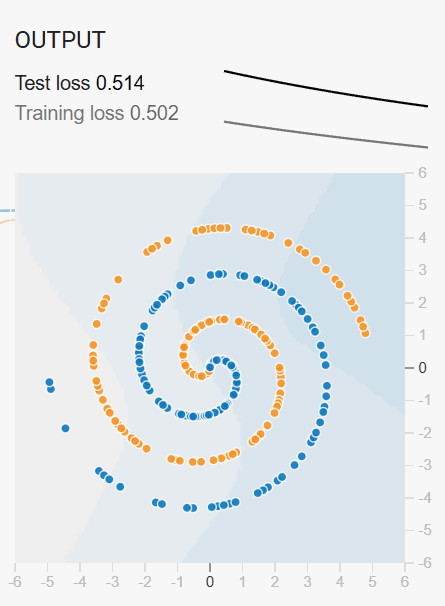
\includegraphics[width=\textwidth]{too-slow-000001.png}
            \caption{学习率过低导致速度过慢}
            \label{fig:step021}
        \end{subfigure}
        \hfill
        \begin{subfigure}[b]{0.3\textwidth}
            \centering
            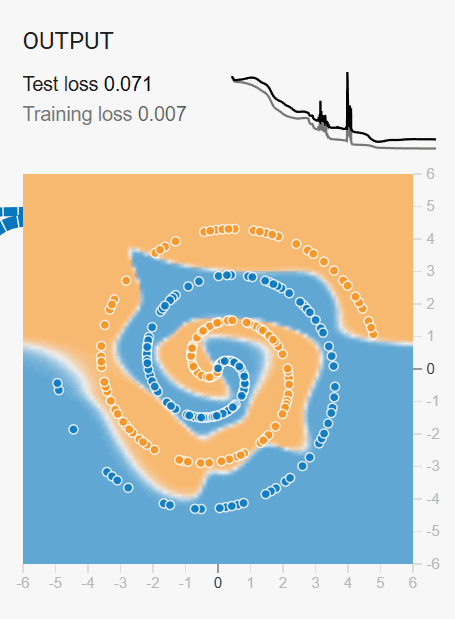
\includegraphics[width=\textwidth]{medium-003.png}
            \caption{学习率适中}
            \label{fig:step086}
        \end{subfigure}
        \hfill
        \begin{subfigure}[b]{0.3\textwidth}
            \centering
            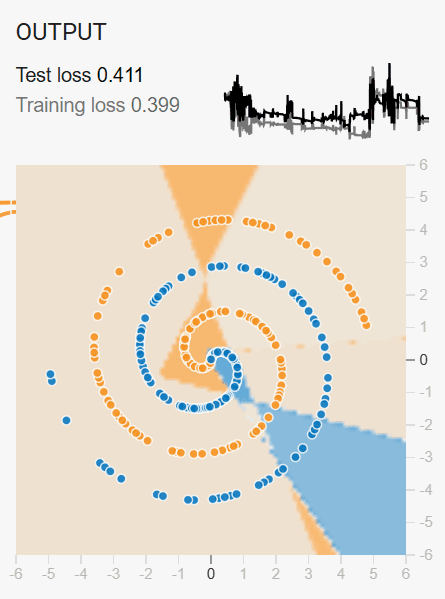
\includegraphics[width=\textwidth]{too-fast-1.png}
            \caption{学习率过大导致损失函数抖动}
            \label{fig:another}
        \end{subfigure}
        \caption{学习率的选择对输出结果的影响}
        \label{fig:comparison}
    \end{figure}


    \subsection{梯度下降法的变种}
    随着梯度下降法在实践中的广泛应用,出现了许多变种算法,以解决其原始形式的一些缺陷。这些变种包括:
    \begin{itemize}
        \item 随机梯度下降($Stochastic\ Gradient\ Descent,\ SGD$):每次迭代仅使用一个样本来更新梯度,适用于大规模数据集。
        \item 小批量梯度下降($Mini-batch\ Gradient\ Descent$):每次迭代使用一小批样本来更新梯度,兼顾了批量梯度下降和随机梯度下降的优点。
        \item 动量梯度下降($Momentum\ Gradient\ Descent$):引入动量项,减少迭代过程中的震荡,加速收敛。
        \item 自适应学习率方法($如AdaGrad,\ RMSprop,\ Adam$):根据梯度信息动态调整学习率,提高收敛效率。
    \end{itemize}


    \section{数学概念/方法中蕴含的数学思维}
    梯度下降法不仅是一种具体的算法, 更蕴含了深刻的数学思维和方法, 这些思维和方法在数学优化和机器学习领域都有着广泛的应用。

    \subsection{优化思维}
    梯度下降法的核心是优化问题, 即在一定条件下找到函数的极小值。优化思维贯穿于整个算法中, 包括目标函数的构建, 学习率的选择, 以及收敛性的分析。

    \subsection{微积分思维}
    梯度下降法依赖于函数的导数和梯度信息, 这些都是微积分的基本概念。通过计算梯度并沿梯度的反方向移动, 我们能够逐步逼近函数的极小值点, 这是微积分在优化问题中的一种具体应用。

    \subsection{迭代思维}
    梯度下降法是一种迭代算法, 通过反复更新变量的值来逼近最优解。迭代思维要求我们在每一步更新中都要考虑当前的梯度信息, 并合理调整步长, 以确保算法的收敛性和效率。
    如下所示:我们使用网站:
    \href{https://fa.bianp.net/teaching/2018/COMP-652/gradient_descent.html}{Fabianp} 来控制调整步长,以便更好地理解梯度下降法的工作原理。
    \begin{figure} [H]
        \centering
        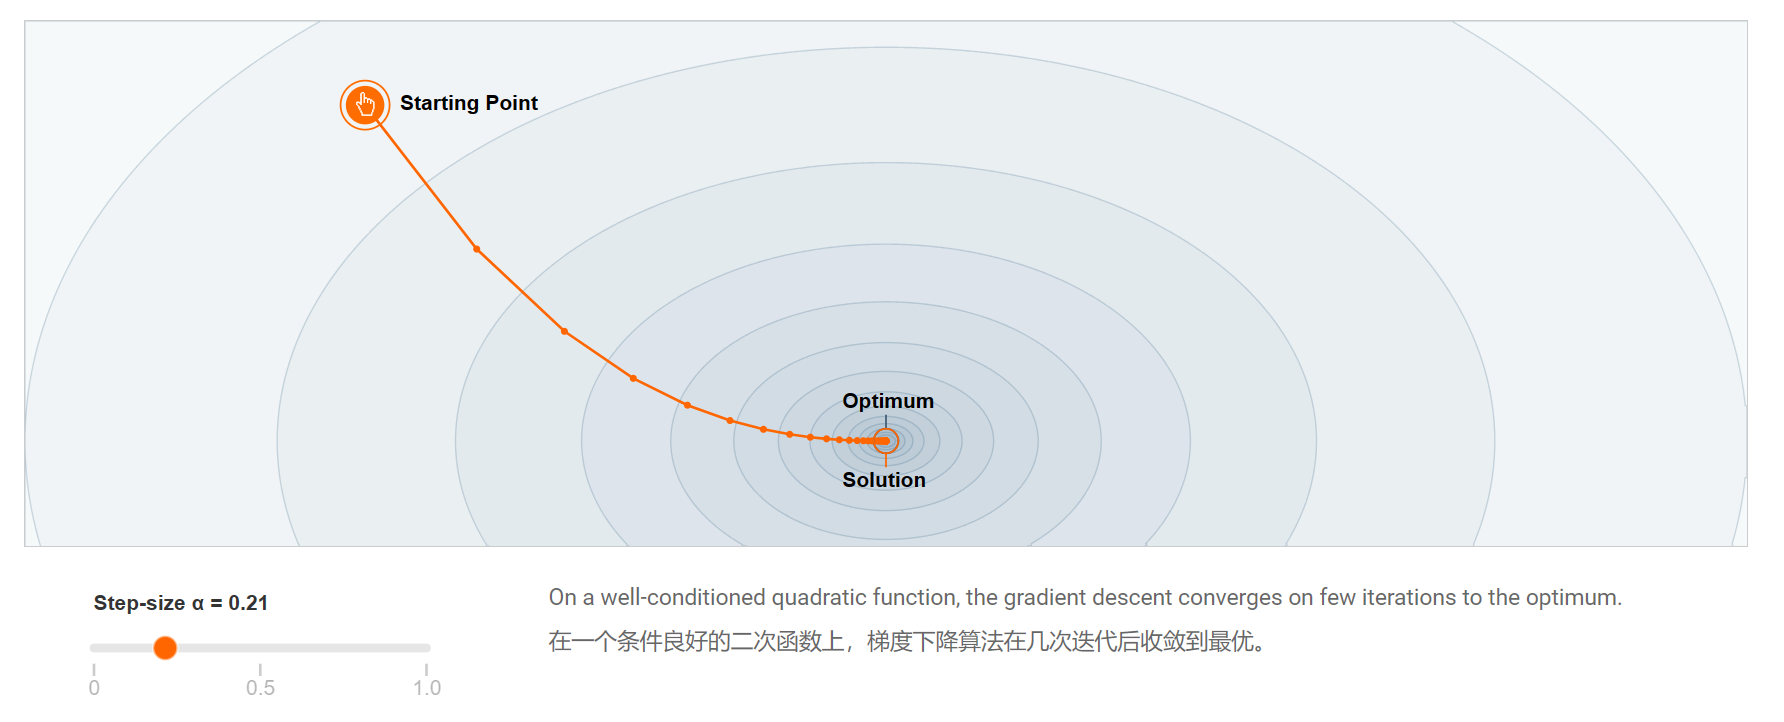
\includegraphics[width=0.95\textwidth]{Step021.png}
        \caption{Step-Size:0.21}
        \label{fig:gradient-descent}
    \end{figure}

    \begin{figure} [H]
        \centering
        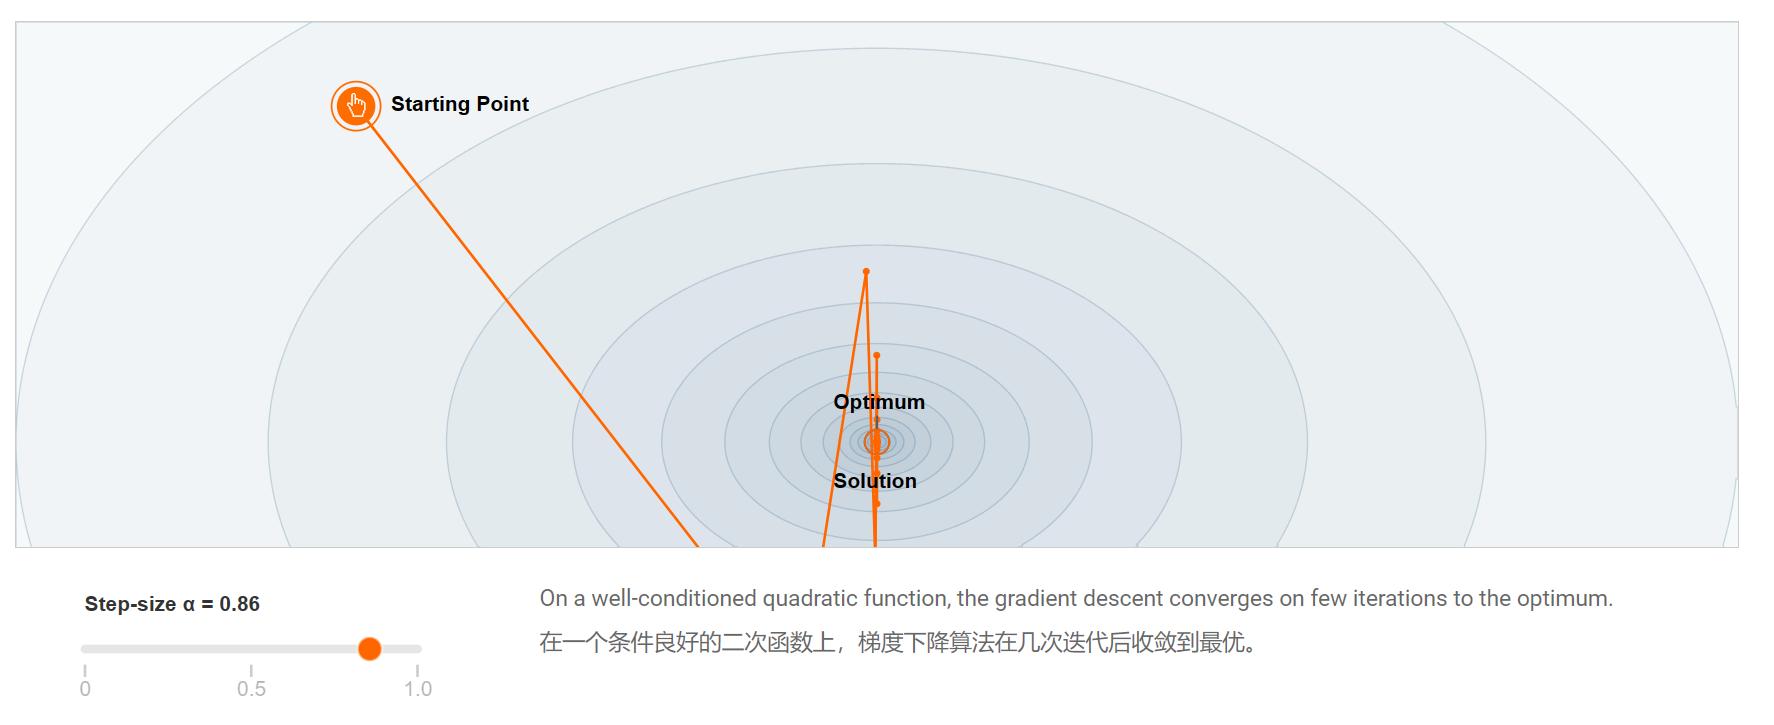
\includegraphics[width=0.95\textwidth]{Step086.png}
        \caption{Step-Size:0.86}
        \label{fig:gradient-descent}
    \end{figure}

    在后图中,步长较大($0.86$),算法在每次更新时跨越的距离较大,容易在损失函数的不同区域之间来回振荡,甚至可能偏离最优解。
    图中可以看到,迭代路径出现了大幅度的跳动,且在最优解附近有明显的振荡,虽然最终也收敛到最优解,但收敛过程不稳定。
    因此,后人们使用了许多算法,步长的选择需要在过小和过大之间找到平衡,以确保收敛速度和稳定性。
    一般可以通过实验或使用自适应步长算法(如$AdaGrad、RMSprop、Adam$等)来优化步长选择。

    这一部分见后文中介绍的内容。

    \subsection{数值分析思维}
    在实际应用中, 梯度下降法需要处理各种数值问题, 如梯度计算的精度, 学习率的选择, 以及算法的收敛速度等。数值分析思维帮助我们在实现和应用梯度下降法时, 解决这些实际问题, 提高算法的稳定性和效率。


    \section{研究背景,即数学概念/方法提出的历史原因}

    梯度下降法的提出和发展有着深刻的历史背景和原因。理解这些背景有助于我们更好地把握这一数学概念和方法的意义及其应用。

    \subsection{早期优化问题的研究}
    在19世纪中叶, 随着微积分和变分法的发展, 数学家们开始关注如何求解复杂函数的极值问题。考克斯($Augustin-Louis\ Cauchy$)于$1847$年提出了梯度下降法, 作为求解这些问题的一种有效方法。这一时期的研究主要集中在理论层面, 探讨了函数极值的性质及其计算方法。

    \subsection{计算机的发展}
    20世纪中叶, 随着电子计算机的发明和发展, 数值计算成为可能。梯度下降法作为一种数值优化算法, 逐渐在计算机科学中得到应用。计算机的高速计算能力使得梯度下降法能够处理大规模的优化问题, 推动了该方法的实际应用和进一步发展。

    \subsection{机器学习的兴起}
    20世纪末至21世纪初, 机器学习迅速发展成为一门重要的学科。梯度下降法作为机器学习模型训练中的核心算法之一, 得到了广泛应用。尤其在神经网络和深度学习领域, 梯度下降法被用来优化模型参数, 从而提高模型的性能。这一时期, 各种梯度下降法的变种(如随机梯度下降, 动量梯度下降, 自适应学习率方法等)也相继被提出和应用, 进一步丰富了梯度下降法的理论和实践。

    \subsection{大数据和人工智能的推动}
    进入21世纪, 大数据和人工智能的蓬勃发展对梯度下降法提出了新的挑战和需求。面对海量数据和复杂模型, 传统的梯度下降法在计算效率和收敛性方面遇到了一些问题。为此, 研究者们提出了一系列改进和优化策略, 如分布式梯度下降, 并行计算等, 以适应大规模数据处理的需求。

    \subsection{多学科交叉的影响}
    梯度下降法不仅在数学和计算机科学中发挥重要作用, 还与物理学, 工程学, 经济学等多个学科紧密相关。不同领域的问题和需求推动了梯度下降法的不断发展和完善, 使其在理论和应用上都取得了显著的进步。
    梯度下降法的提出和发展有着深厚的历史背景和多方面的推动因素。从早期的理论研究到现代的广泛应用, 梯度下降法不断演进, 成为解决优化问题的重要工具。


    \section{概念/方法的不断改进和发展}

    随着时间的推移和技术的发展, 梯度下降法不断地被改进和发展, 以满足不同应用场景的需求。

    \subsection{随机梯度下降法($SGD$)}
    传统的梯度下降法每次迭代都会使用整个数据集计算梯度, 对于大规模数据集, 这种方法计算量大且效率低。随机梯度下降法($SGD$)通过在每次迭代中随机选取一个样本来更新梯度, 大大提高了计算效率。

    在研究$SGD$随机梯度下降算法时,我们通过研究最典型的$SGD$代码实现,来更好地理解$SGD$的工作原理。

    \begin{lstlisting}[language = python, title = {$SGD\ Algorithm$}]
        import torch
        from torch import nn, optim
        
        # 定义一个简单的线性模型
        model = nn.Linear(2, 1)  # 输入2个特征, 输出1个值
        
        # 假设有输入数据和标签
        inputs = torch.randn(100, 2)  # 100个样本, 每个样本2个特征
        labels = torch.randn(100, 1)  # 100个样本, 每个样本1个标签
        
        # 创建优化器, 指定要更新的模型参数
        optimizer = optim.SGD(model.parameters(), lr=0.01)  # 学习率为0.01
        outputs = model(inputs)                        # 前向传播
        loss = nn.MSELoss()(outputs, labels)           # 损失函数
        loss.backward()                                # 反向传播并计算梯度
        optimizer.step()                               # 使用优化器更新参数
        optimizer.zero_grad()                          # 清除梯度(防止梯度累积)
    \end{lstlisting}

    在运行代码时, 我们使用了zero\_grad来清除梯度, 为何要进行最后的这一步操作呢?
    在学习的过程中,
    我们了解到:

    ``梯度累积''指: 多个批次或样本上计算梯度时, 将梯度相加累积的情况.
    梯度累积会导致参数更新步骤推迟,
    尤其是在训练过程中使用较大的学习率时.
    较大的梯度可能导致模型参数跳跃到不良的局部最小值或发散的情况.
    因为只有在清除梯度后, 才能执行参数更新.
    这可能导致梯度更新的频率降低, 从而延缓模型的收敛速度.

    那么, 没有$optimizer.zero\_grad()$会发生什么呢?

    为了可视化相关的结果,
    我们学习使用了$matplotlib$库来体现两者的差别.
    $Python$代码如下所示:

    \begin{lstlisting} [language = python, title = {Visualization} ]
        import torch
        from torch import nn, optim
        import matplotlib.pyplot as plt

        # 定义一个简单的线性模型
        model1 = nn.Linear(2, 1)  # 模型1
        model2 = nn.Linear(2, 1)  # 模型2

        # 假设有输入数据和标签
        inputs = torch.randn(100, 2)  # 10个样本,每个样本2个特征
        labels = torch.randn(100, 1)  # 10个样本,每个样本1个标签

        # 创建优化器
        optimizer1 = optim.SGD(model1.parameters(), lr=0.01)
        optimizer2 = optim.SGD(model2.parameters(), lr=0.01)

        # 用于记录损失
        losses_with_clear_grad = []
        losses_without_clear_grad = []

        # 训练100个步骤,清除梯度的情况
        for step in range(100):
            outputs = model1(inputs)
            loss = nn.MSELoss()(outputs, labels)
            losses_with_clear_grad.append(loss.item())

            optimizer1.zero_grad()  # 清除梯度
            loss.backward()
            optimizer1.step()

        # 训练100个步骤,不清除梯度的情况
        for step in range(100):
            outputs = model2(inputs)
            loss = nn.MSELoss()(outputs, labels)
            losses_without_clear_grad.append(loss.item())

            # 这里没有调用 zero_grad()
            loss.backward()
            optimizer2.step()

        # 可视化对比
        plt.plot(range(100), losses_with_clear_grad, marker='o', label='With Clear Gradients')
        plt.plot(range(100), losses_without_clear_grad, marker='x', label='Without Clear Gradients')
        plt.xlabel('Step')
        plt.ylabel('Loss')
        plt.title('Loss during Training')
        plt.legend()
        plt.show()
    \end{lstlisting}

    含有梯度清除和不含梯度清除时, 两者的差别如下图所示:

    \begin{figure} [H]
        \centering
        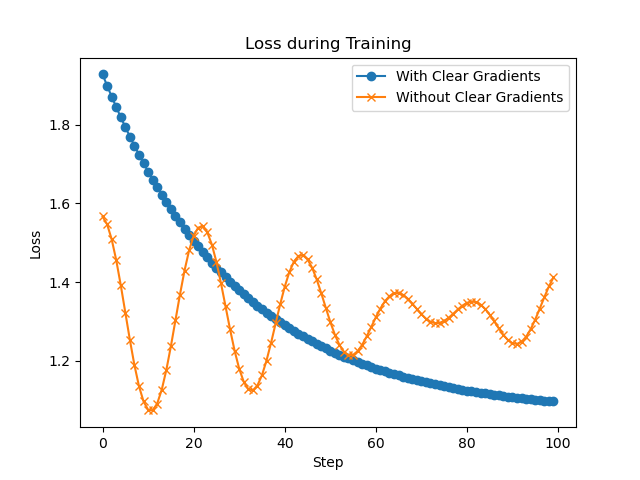
\includegraphics[width=0.6\textwidth]{../lectures/img/clear-gradients.png}
        \caption{梯度清除与不清除的损失对比}
    \end{figure}

    在每个批次或样本的反向传播之后, 及时清除梯度, 确保每个批次的梯度都是独立计算的.
    如果梯度累积导致模型不稳定或训练速度过慢, 减小学习率也可以降低梯度的影响.

    \subsection{小批量梯度下降法}
    小批量梯度下降法($Mini-batch\ Gradient\ Descent$)结合了批量梯度下降和随机梯度下降的优点, 每次迭代使用一个小批量的样本来更新梯度, 既保证了计算效率, 又平滑了梯度的更新过程, 提高了算法的稳定性。


    \section{动量 ($Momentum$)}

    随机梯度下降 ($SGD$) 对计算梯度时数据的计算批次进行优化, 但是面对特殊的损失函数的值, $SGD$ 会出现梯度缺失, 更新停滞的问题。例如, 在马鞍面形状的损失函数图像上进行梯度下降, 如图所示, 可能会导致梯度下降的步伐在马鞍面的凸起方向反复徘徊, 而难以进一步降低损失函数的值。

    \begin{figure}[H]
        \centering
        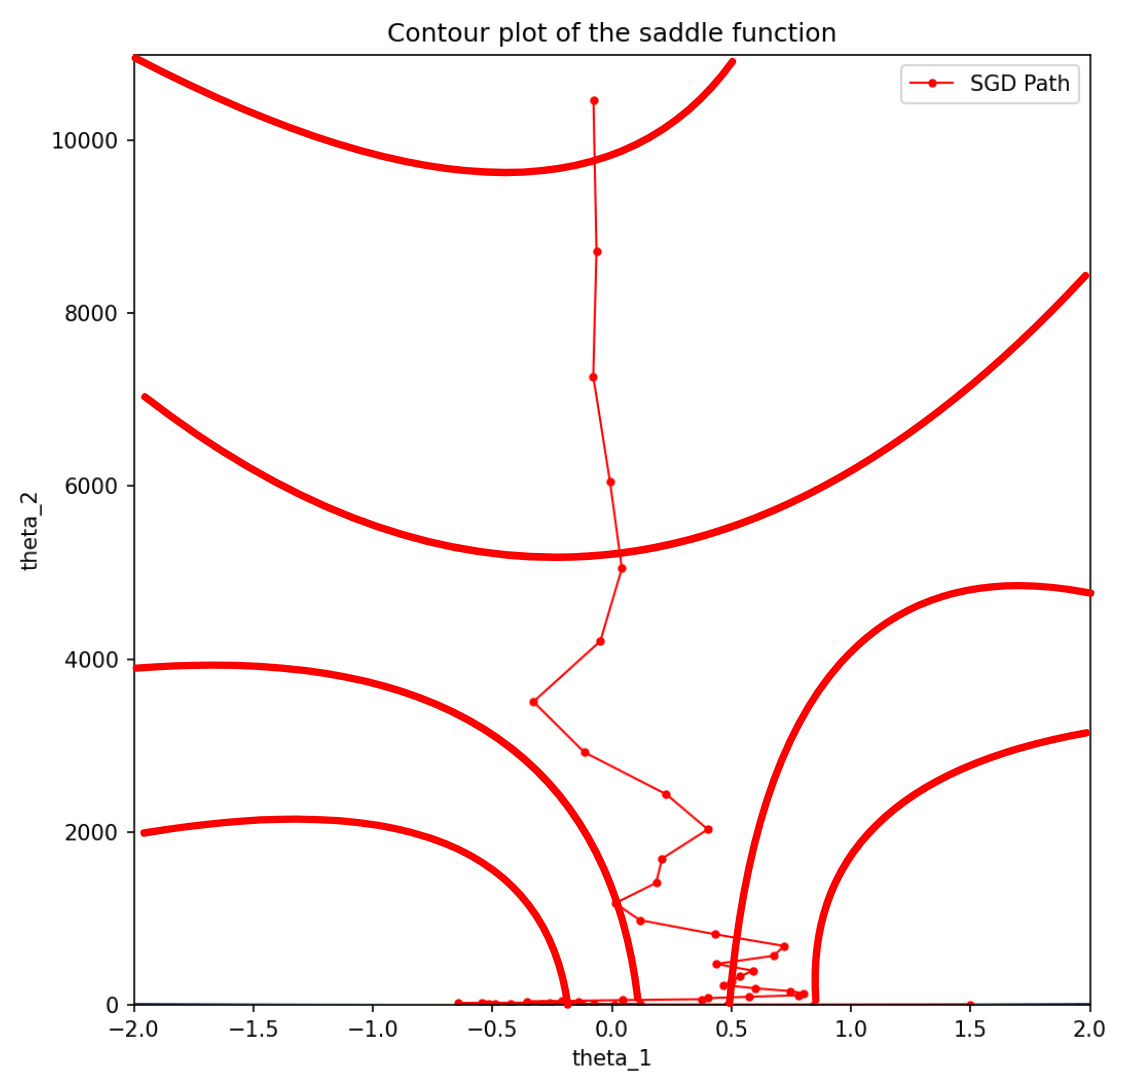
\includegraphics[width=0.7\textwidth]{../lectures/img/saddle-no-momentum-sgd.jpg}
        \caption{在马鞍面上的随机梯度下降}
    \end{figure}

    在上图中, 随机梯度下降由于马鞍面的形状而在一开始缓慢下降, 效率低下。
    于是动量 ($Momentum$) 的概念被引入, 它用于在梯度下降时提供一个由积累而产生的向量值。动量在梯度下降时不断震荡, 徘徊的方向上会不断抵消, 而在稳定缓慢前进的方向上会不断累加, 这个方向上的动量的累加有利于梯度下降更加快地跳出如马鞍面的图形中的鞍点中的区域。
    具体运算步骤如下:

    \begin{figure}[H]
        \centering
        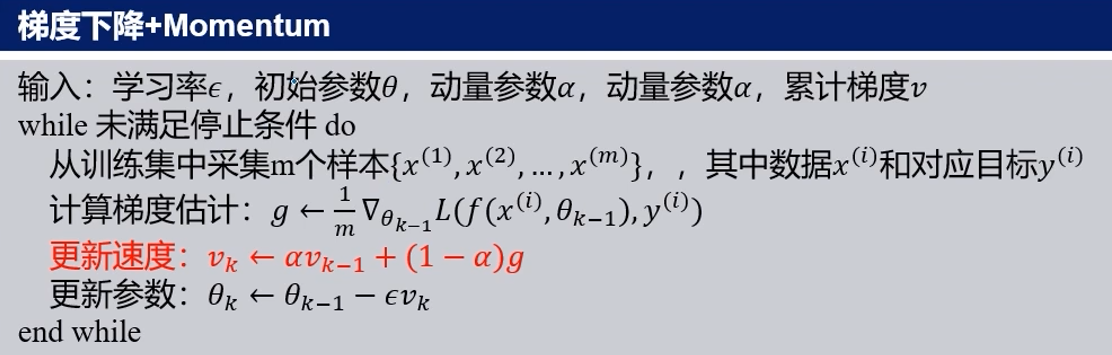
\includegraphics[width=0.7\textwidth]{../lectures/img/gd-with-momentum.jpg}
        \caption{动量梯度下降的步骤}
    \end{figure}

    红色字体的部分展现了动量累积的步骤, 其通过前次动量和当次梯度来累积动量, 其中 \( v \) 是动量, \( \alpha \) 作为动量参数, 在动量更新时起到了保留多少比例的前次动量的作用, 换句话说 \( 1 - \alpha \) 便影响了动量更新的速度。


    \section{$Adagrad$}

    除了调整动量这一方法, 另外一种思路是自适应调整梯度 ($Adagrad$), 它根据参数调整学习率, 针对与频繁出现的特征相关的参数执行更小的更新 (即低学习率), 针对与不频繁的特征相关的参数执行更大的更新 (即高学习率)。一种更加通俗的理解是此算法能做到在震荡的地方步长很小, 而在梯度较小的地方步长变大。
    简要的运算步骤如下:

    \begin{figure}[H]
        \centering
        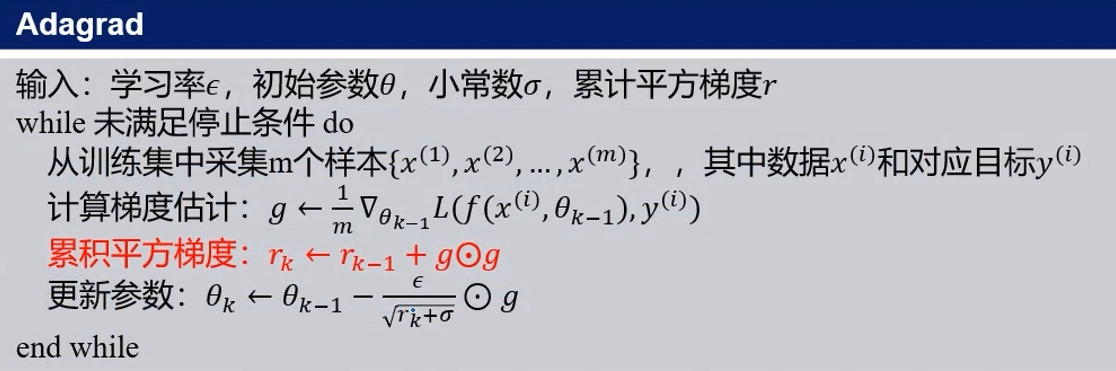
\includegraphics[width=0.7\textwidth]{../lectures/img/adagrad-steps.png}
        \caption{$Adagrad$的运算步骤}
    \end{figure}

    在累积平方梯度时, 如果梯度的平方较大, 那么在下一步更新参数时, 第二项的分母越小, 从而实现梯度的自适应。
    特别的是, 在累积平方梯度这一步时, 不是简单地将原来的平方梯度和新的平方梯度相加, 而是在它们之间添加一个比例参数, 类似 Momentum 中的 \( \alpha \), 这便是 \textbf{RMSProp}。


    \section{$Adam$}

    $Adam$ 集合了 $Momentum$ 和 $RMSProp$ 两个的思路, 综合了动量和自适应的优点, 避免了冷启动的问题。
    经验表明, $Adam$ 在实践中表现很好, 和其他适应性学习算法相比也比较不错。
    简要步骤如下:

    \begin{figure} [H]
        \centering
        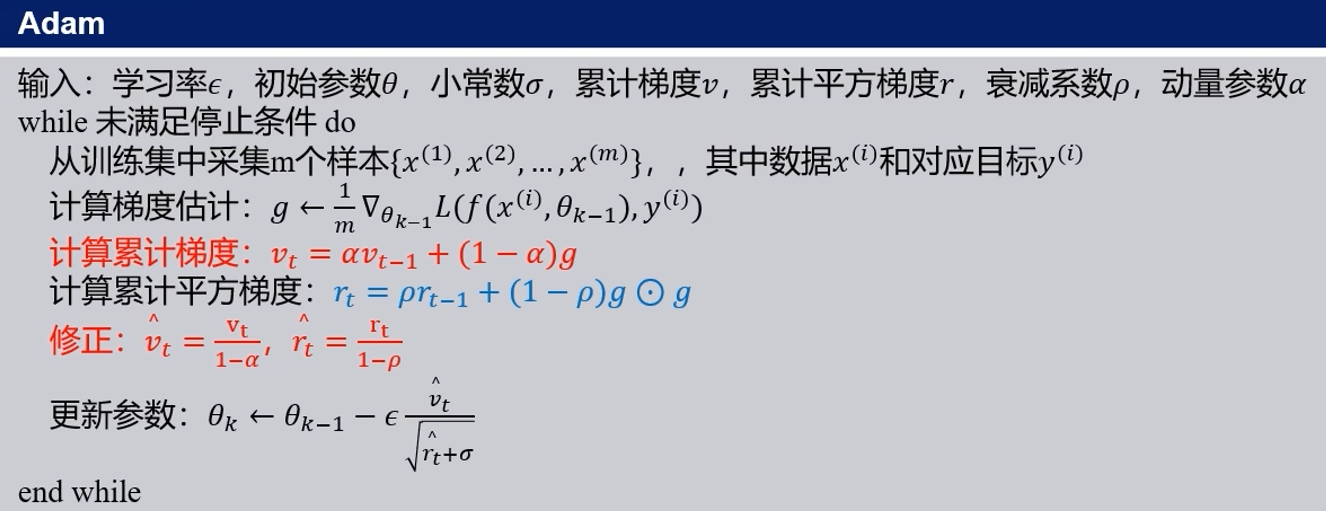
\includegraphics[width=0.7\textwidth]{../lectures/img/adam-steps}
        \caption{$Adam$的运算步骤}
    \end{figure}

    在我们的学习中,可以知道其代码实现如下:

    \begin{lstlisting} [language = python, title = {Adam Algorithm}]
    optimizer = optim.Adam(model.parameters(), lr=0.001, betas=(0.9, 0.999))
    \end{lstlisting}

    \section{概念/方法的应用现状}

    \subsection{应用领域}
    梯度下降法在多个领域中有广泛应用。首先,在机器学习和深度学习中,梯度下降法用于优化模型参数,使得模型对训练数据的误差最小。其次,在经济学和金融学中,梯度下降法用于优化投资组合和风险管理。最后,在工程和物理学中,梯度下降法用于优化复杂系统的控制参数。

    \subsection{实际案例}
    一个实际的应用案例是$Google$的神经机器翻译系统($GNMT$),该系统利用梯度下降法来训练其深度神经网络,从而大幅提高翻译的准确性。另一个案例是自动驾驶汽车,特斯拉的自动驾驶系统利用梯度下降法不断优化其算法,以实现更安全和更高效的驾驶体验。

    \subsection{未来发展方向}
    未来,梯度下降法将在更多领域中发挥重要作用。例如,在生物医学领域,梯度下降法将用于优化基因编辑和药物发现。此外,随着量子计算的发展,梯度下降法可能会结合量子算法,实现更快速和更高效的优化过程。

    \chapter{通过此选题的调研和分析所产生的体会和启发}

    通过本次对梯度下降法的调研和分析,我深刻体会到了其在不同领域中的广泛应用和重要性。调研过程中,我不仅深入了解了梯度下降法的基本原理和变种算法,还通过实际案例进一步理解了其在实际问题解决中的强大功能。同时,通过对比不同优化算法,我意识到在选择合适的算法时需要综合考虑数据的特性和应用场景。此外,通过本次调研,我也学会了如何使用LateX进行科学报告的撰写,提高了我的科研写作能力。


    \section{调研和分析的过程}
    本次调研和分析的过程分为以下几个阶段:

    \subsection{选题确定}
    在调研初期,我们小组讨论了多个可能的选题,包括猫狗识别、手势识别等人工智能模型的建立,以及$CNN$、梯度下降等算法的学习方面。最终,我们选择了梯度下降法作为我们的研究主题,因为梯度下降法是人工智能中最基础和最重要的算法之一。

    \subsection{资料收集}
    确定选题后,我们开始收集相关资料。我们通过阅读吴恩达的机器学习课程、查阅相关论文和书籍,以及观看在线教程,全面了解了梯度下降法的基本原理、变种算法以及其在不同领域的应用。

    \subsection{算法研究}
    在资料收集的基础上,我们对梯度下降法及其变种算法(如随机梯度下降法、动量法、$Adagrad$、$Adam$等)进行了深入研究。通过编写和运行实际代码,我们理解了这些算法的实现细节和优缺点,并通过实验验证了不同算法在不同数据集上的表现。

    \subsection{报告撰写}
    在研究和实验的基础上,我们撰写了本次课程报告。报告内容包括梯度下降法的基本概念、变种算法、应用现状以及实际案例分析。撰写过程中,我们还学习和使用了LateX进行排版,使得报告格式规范、美观。

    \subsection{总结与反思}
    通过本次调研和分析,我们不仅深入了解了梯度下降法,还学会了如何进行科学研究和报告撰写。我们认识到选择合适的优化算法需要综合考虑多个因素,如数据特性、计算资源和应用需求。同时,我们也意识到在科学研究中,理论与实践的结合至关重要。未来,我们将继续关注和学习更多前沿算法,进一步提升我们的科研能力。


% 声明后置部分开始
    \backmatter

% 致谢
    \begin{acknowledgement}
        \begin{itemize}
            \item 张梓卫:

            \begin{itemize}
                \item 组长,PPT 后续排版与校对、课程报告 $LateX$ 排版、课程报告中 $SGD$ 实例代码提供、组织小组合作。
                \item 通过本次的人工智能的数学思维的报告编写,我们从选题到最终定稿,花费的周期大约在一个月,期间,
                我们选择了猫狗识别、手势识别等人工智能模型的建立,以及$CNN$、梯度下降等算法的学习方面作为题材。
                但最后我们选择了梯度下降法作为我们的选题,因为梯度下降法是人工智能中最基础的算法之一,也是最重要的算法之一。
                通过这次的报告,我们先从吴恩达的机器学习开始学起,后来我又在一些网课教程中找到了$CNN$学习到了梯度下降法的基本原理,以及梯度下降法的变种,如随机梯度下降法、动量法、$Adagrad$、$Adam$等。
                更重要的是,我学会了使用LateX的本科生毕业论文的模板,我修改了部分参数,使得整个模板能够适配课程报告论文。
            \end{itemize}

            \item 关卓谦:

            \begin{itemize}
                \item 深度学习主要框架搭建、课程报告主体框架与主要内容编写、提供公式及图片、为课程报告中自建模型的代码的编写者。
                \item 通过对深度学习的学习, 我深刻体会到了梯度下降这项算法的简洁与强大.
                梯度下降通过简单的负梯度更新方法, 在解决复杂优化问题时展现了极大的威力.
                选择合适的学习率需要在速度和稳定性之间找到平衡, 这让我意识到数据科学中的很多问题实际上是平衡与取舍的艺术.
                此外, 梯度下降的多种变种, 如动量和$Adam$, 展示了其适应不同数据和模型需求的能力.
                通过实际代码实现和实验调优, 我深刻理解了理论与实践的紧密联系, 也对算法设计者的智慧心怀敬畏.
                尽管梯度下降已经广泛应用, 我仍期待未来能有更多创新算法出现, 进一步推动人工智能的发展.
                总之, 梯度下降不仅是一种数学工具, 更是一扇通往更广阔科学世界的窗口.
            \end{itemize}

            \item 周诗泽:

            \begin{itemize}
                \item 负责$PPT$的前置制作、课程报告中“追本溯源”与“应用效果编写”。
                \item 通过本次报告的编写,我深入了解了梯度下降法的起源与应用。作为负责“追本溯源”部分的我,
                从历史的角度出发,回顾了梯度下降法的发展历程,展示了其在不同领域中的广泛应用。
                我在$PPT$制作中,注重将复杂的算法原理以简洁明了的方式呈现。这次合作让我深刻体会到了团队协作的重要性,
                每个人的努力都汇聚成了最终的成果。感谢组长张梓卫的指导和关卓谦的技术支持,我们共同完成了这份具有深度和广度的课程报告。
            \end{itemize}
        \end{itemize}
    \end{acknowledgement}

% % 打印参考文献
% \printbibliography

\newpage
\section*{参考文献}
\begin{itemize}
    \item Wikipedia, \textit{Gradient Descent}, \url{https://en.wikipedia.org/wiki/Gradient_descent}, 访问时间:2023年6月9日.
    \item 作者: 知乎用户, \textit{机器学习——从输入到输出}, 2023, \url{https://zhuanlan.zhihu.com/p/580645925}, 访问时间:2023年6月9日.
    \item Pierre Baldi, \textit{Gradient descent learning algorithm overview: A general dynamical systems perspective}, IEEE Transactions on neural networks, 1995, 6(1): 182--195.
    \item Shun-ichi Amari, \textit{Backpropagation and stochastic gradient descent method}, Neurocomputing, 1993, 5(4-5): 185--196.
    \item Florian Schäfer and Anima Anandkumar, \textit{Competitive gradient descent}, Advances in Neural Information Processing Systems, 2019, 32.
\end{itemize}

\end{document}